\section{Introduction} % A complete overview

% DONE Introduces the larger reasearch area that the paper is part of
% DONE Illustrates the concrete problem
% Explains the proposed solution
% Highlights the main results
% Might finish with a short explanation of the following sections

In computer architecture, the ``memory wall''~\cite{wulf_mckee_1995}
is a well known problem. Slow memory act as a bottleneck in a system
with fast processors. The reason for this is that processors will
request data faster than what primary memory can provide. In a Von
Neumann architecture\todo{find article to cite here}, the processor
will stall as it waits for the next data or instruction to arrive.

There are several techniques used in modern systems which mitigates
this bottleneck, like caching, outsourcing memory management to a DMA,
branch predictions, etc. One interesting approach is named
``prefetching''.

Prefetching involves speculating in which memory
addresses are needed in the near future, and fetching them prior to
execution. This paper investigates the ``speculating'' part, that is,
what addresses should we fetch and when. When the prefetching is
successful, we avoid CPU stalling as the processor has the needed data
available and we get increased performance. When we are unsuccessful,
we waste valuable cache space.

The most basic kind of prefetching would be to load the memory
addresses which sequentially follow the address we are currently
working on. However, this tends to be not so effective as memory
access tend to be non-sequential. Instead, we can look for access
patterns, and try to exploit them.

Our approach does this by using a reference prediction table.
In this paper we analyse the result of a basic implmentation of RPT,
and we show how to improve RPT using a lookahead technique.

% \begin{center}
% 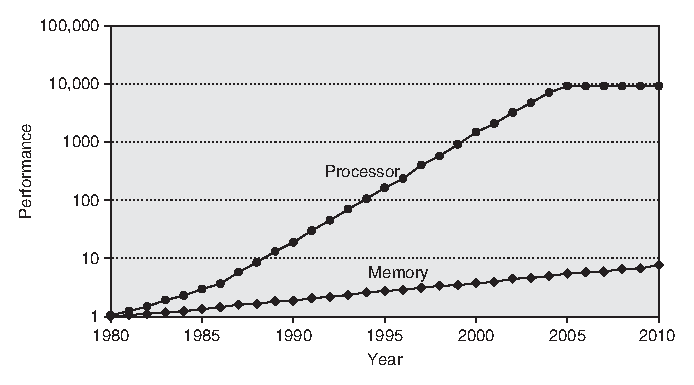
\includegraphics[width=0.5\textwidth]{graphs/memorywall}
% \end{center}

% http://ieeexplore.ieee.org/abstract/document/5389383/
